%!TEX root = ../../main.tex
\subsection{Pre Test} \label{ssec:pretest}
This chapter describes the pre-test that is mentioned above.
The chapter will describe the acquisition of data the evaluation of the gathered results.

\subsubsection{Purpose}
The purpose of this pre-test is to test the implementation and test its eligibility for the main testing.
The pre-test will produce observations for use in further development of the implementation and for use in the discussion and re-design.
Because the main test will be conducted on people outside of a lab environment, we want reduce the time required by the test participants.
The ultimate purpose of the pre-test is to establish how many generations are needed for the final test.

\subsubsection{Method}
The pre-test will be conducted with ourselves as subjects and will not require any outside test participants.

The test conductor will run 20 generations of the game and note any observations regarding troubleshooting, initial failures, and missing functionalities.
The data required from the games logs are the genes for the ghosts, the time taken to do a play-through of the game followed by the 10 simulations.
The time will be taken manually by the test conductor.

The observations considered most critical to the conduction of the main test will be attended to during the test and the test will be restarted.

The test will be done under the assumption that as the generations will progress, the alterations on the genes of the ghosts, done by the GA, will start to stabilize.
The point where the genes start to stabilize will be the point where we main test can be terminated.

To find this point the content of the genes are required the average value of the genes per generation, per ghost, per mode.
When the average values will be similar to the previous value over a range of generations, the genes can be considered to be stabilizing.

\subsubsection{Procedure}
\begin{enumerate}
	\item Gather sample and record time.
	\begin{enumerate}
		\item Play game (F1)
		\item Run simulation (F5)
	\end{enumerate}
	\item Note observations and errors.
	\item Copy simulation data (F8)
	\item Gather sample and record time.
	\begin{enumerate}
		\item Play improved game (F9)
		\item Run simulations (F5)
	\end{enumerate}
	\item Note observations and errors
	\item Copy simulation data (F8)
	\item Repeat from step 4
\end{enumerate}

\subsubsection{Results}
The gathered list of observations is listed below.

\subsubsection*{Comments}

\begin{itemize}
	\item Ghosts go together (ghosts have the same movements, making them walk on top of each other)
	\item Ghosts appear to be inactive for too long after power pellet.
	\item When the player dies and the simulations are running, the player continues down the predetermined path until it hits a wall, upon death.
	\item When the player dies during a run, then for the following simulations, upon the time of death of the player, the pac-man becomes idle and is not moving until death occurs.
	\item Ghosts appear to stop moving for a considerable amount of time during simulations.
	\item The blue ghost appear to seek the upper left corner to circulate in several simulations following a somewhat similar pattern.
	\item Some ghosts perform similar movement in several simulations.
	\item When consumed, ghosts spawn instantly on the spawn point, Resulting in instant death if ghost is consumed on this area, resulting in spawning almost simultaneously on the same location.
	\item When ghosts are consumed, they spawn and occasionally don’t move for several seconds from the spawning location.
	\item In simulations where the player died, and therefore is standing still on the location of death, the ghosts seem to move to the upper left corner, where they circulate.
	\item One ghost(orange) didn’t move for almost an entire simulation.
	\item The ghosts loose all sense of “intelligence” when pac-man is standing still and they face the wall.
\end{itemize}

\subsubsection*{Timing}
The table below consists of the time it took to do a player recording together with the following ten simulations and copying the results from that generations test results into a separate document.
\begin{table}[!htbp]
\centering
\begin{tabular}{l c}
generations & Time recorded \\
\hline
1 & 3:15 \\
2 & 2:00 \\
3 & 2:51 \\
4 & 2:47 \\
5 & 1:37 \\
6 & 2:18 \\
7 & 3:19 \\
8 & 2:19 \\
9 & 2:06 \\
10 & 2:55 \\
11 & 4:01 \\
12 & 1:56 \\
13 & 3:33 \\
14 & 2:59 \\
15 & 1:44 \\
16 & 3:22 \\
17 & 2:35 \\
18 & 3:00 \\
19 & 2:21 \\
20 & 3:23 \\
\hline
\end{tabular}
\caption{Times per generation during pre-test}\label{tab:times}
\end{table}

The total time was 54.12

The average play-through took 2.43 minutes.


\subsubsection*{Genes}
The collected gene-data from the logs can be found on the digital appendix.
Below will be the processed data.

\begin{figure}[!htbp]
	\centering
	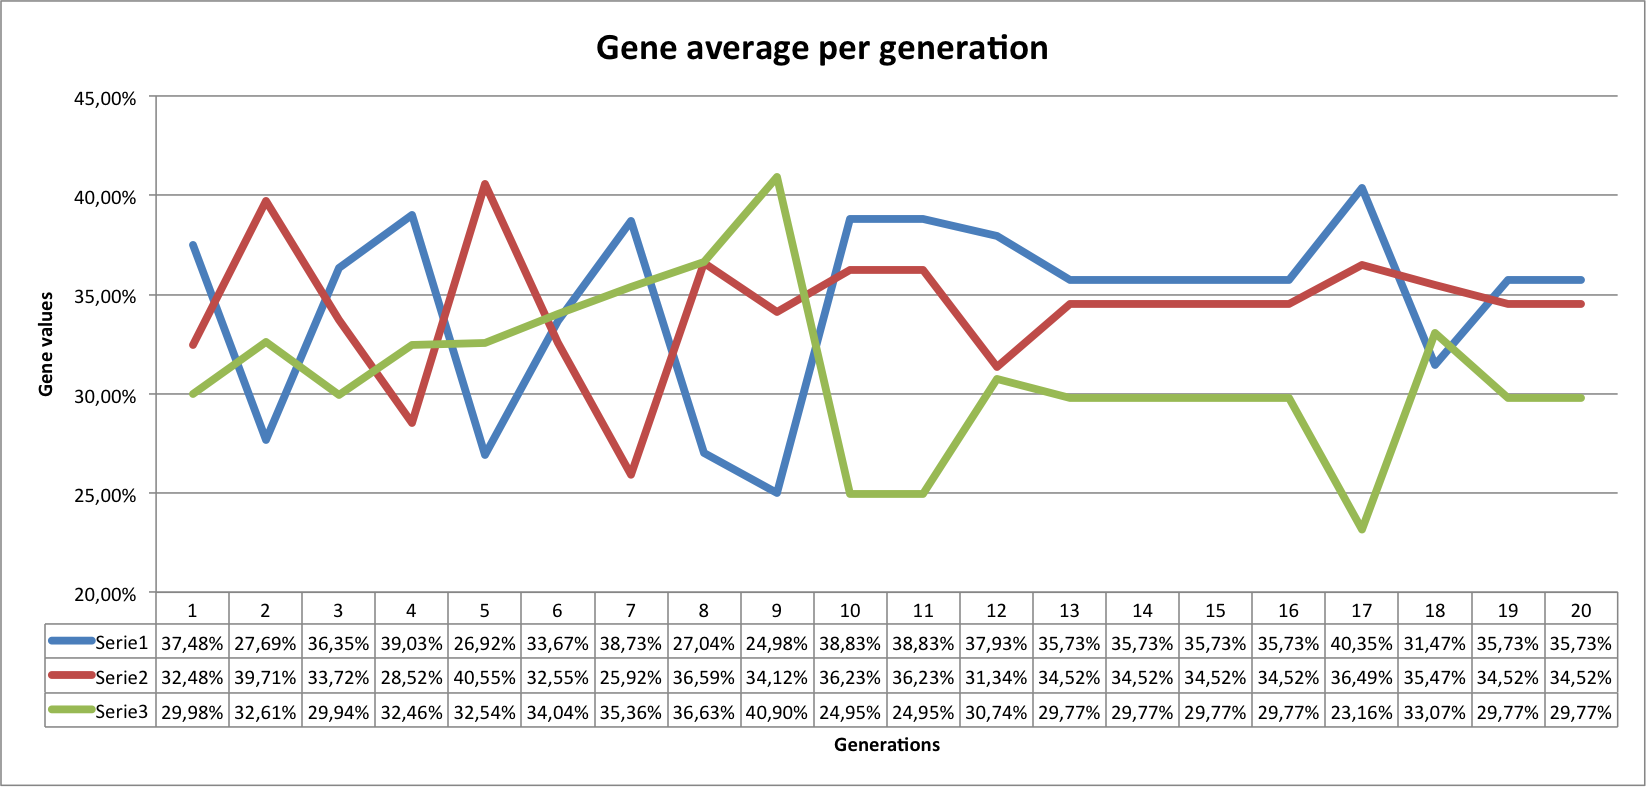
\includegraphics[width=0.85\textwidth]{pretest_average.png}
	\caption{Averages of genes over generations.}
	\label{fig:pretest_average}
\end{figure}

\begin{figure}[!htbp]
	\centering
	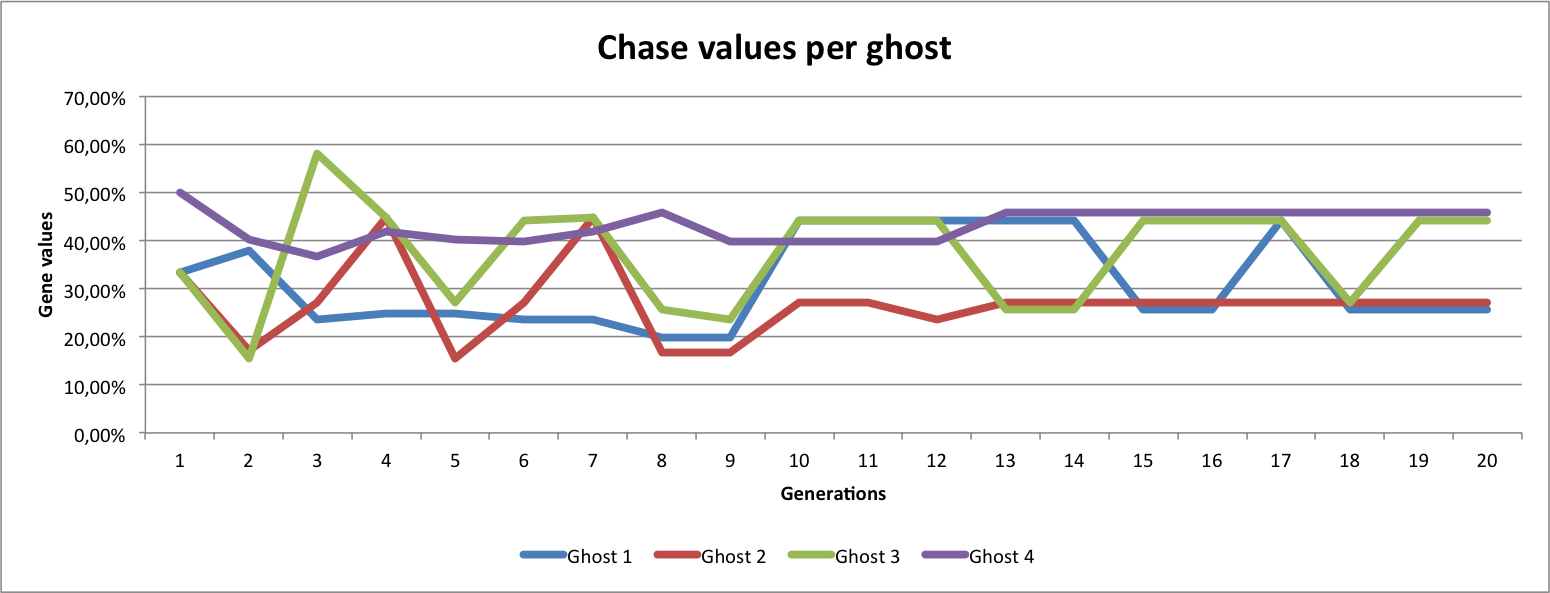
\includegraphics[width=0.75\textwidth]{pretest_chase.png}
	\caption{The recorded chase mode values over generations.}
	\label{fig:pretest_chase}
\end{figure}

\begin{figure}[!htbp]
	\centering
	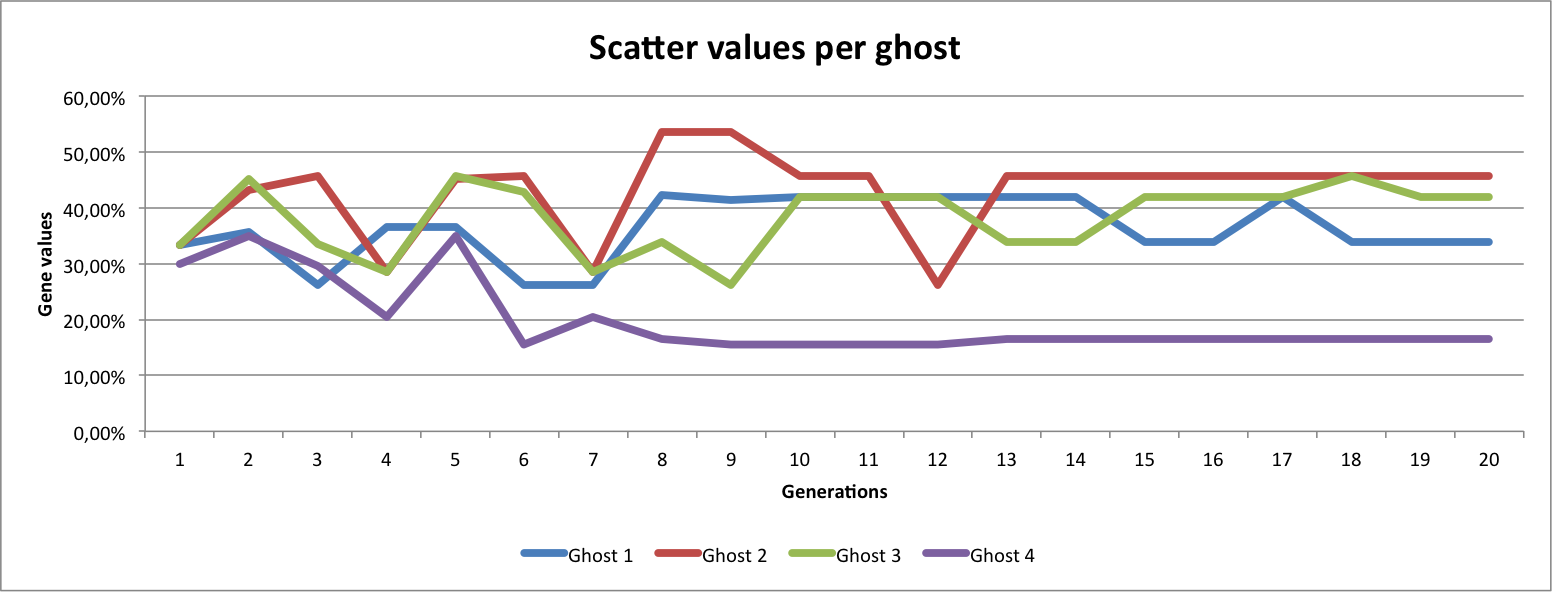
\includegraphics[width=0.75\textwidth]{pretest_scatter.png}
	\caption{The recorded scatter mode values over generations.}
	\label{fig:pretest_scatter}
\end{figure}

\begin{figure}[!htbp]
	\centering
	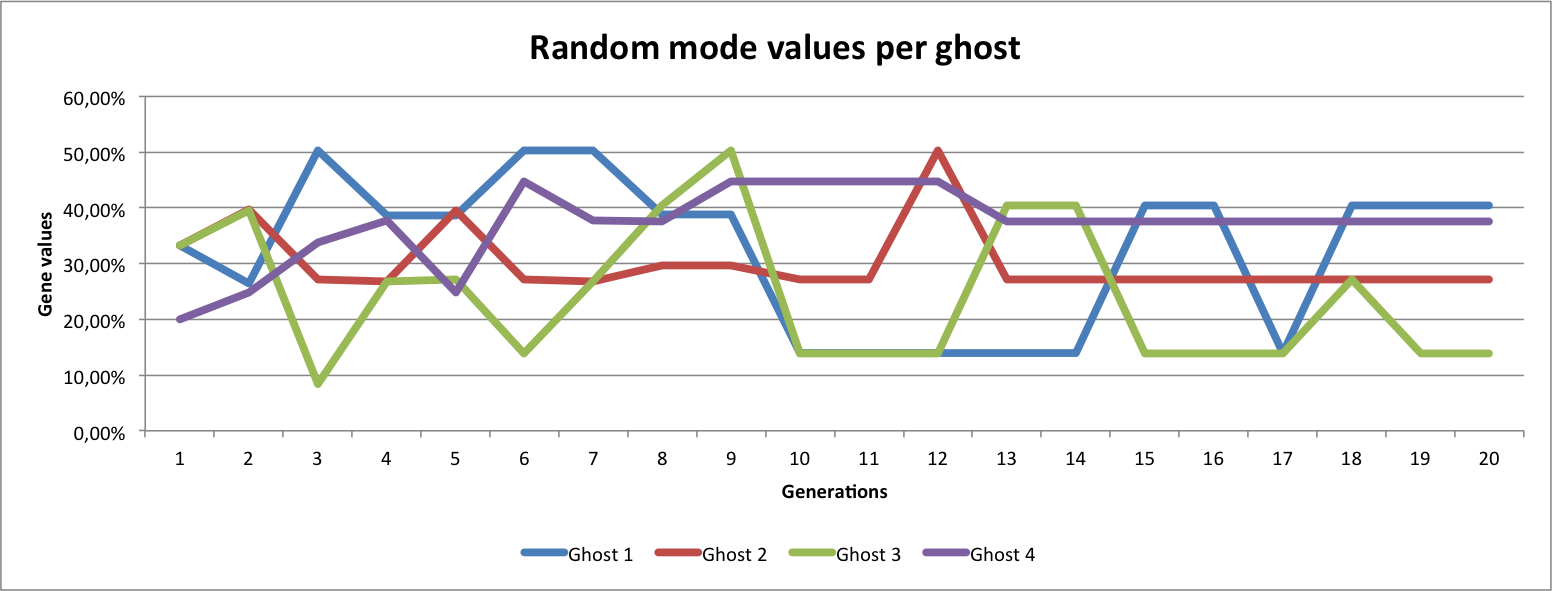
\includegraphics[width=0.75\textwidth]{pretest_random.png}
	\caption{The recorded random mode values over generations.}
	\label{fig:pretest_random}
\end{figure}

\subsubsection{Result Evaluation}
Of the comments shown above, the observation that the ghost spend too long in flee mode was fixed during the testing as it greatly reduced the time the ghosts were active during a game, which can be considered a bias.
The new time the ghosts spend in flee mode is reduced to two and a half seconds.

The ghosts would all gather in the same corner during scatter mode.
This is not intentional and was fixed during testing.
The ghosts now go to a separate corner of the maze during scatter mode.

\subsubsection*{Genes}
By analyzing the genes we want to find the point where the genes start to stabilize and the variations in the genes do not vary.
This point is considered where the GA can no longer make alterations that can match the player performance any better than what it already has.
At this point we speculate that the values of the genes will not be altered any further.
The user test should be terminated at this point.

Figure~\ref{fig:pretest_average} shows average values of the genes for each mode for each ghost in each generation.
If the average is the same as the previous value it means that the sum of the genes values for each ghost in that generation has not changed in the new generation.
This could mean that the genes are unchanged or swapped within the same generation.

It can be seen on figure~\ref{fig:pretest_average} that the genes start to stabilize shortly after the tenth generation with only a few spikes in the averages.

In figures~\ref{fig:pretest_chase},~\ref{fig:pretest_scatter}, and~\ref{fig:pretest_random} the values of a specific mode within the genes are placed up against their generations.
These also indicate that the genes start to stabilize around the tenth generation with only few variations within the range of the lowest and highest values.

\subsubsection*{Time}
Because we will be conducting the test on random sampled participants without appointment we want to minimize the amount of time needed by the participant.
We see 30 minutes as being an acceptable timeframe to ask of people for the test.

It is seen in the results that a test with 20 generations will take around 54 minutes, which means that we can do 11 generations within 30 minutes.
Together with the results from the gene comparison above, which suggests that the genes will stabilize around generation 10, we estimate that 10 generations will be adequate for the each test participant.